
\section{Prädikatenlogik: Semantik}

\begin{frame}{Interpretation}
	\begin{figure}[h!]
		\centering
		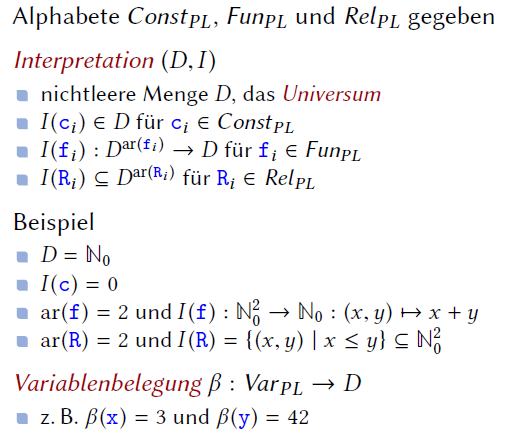
\includegraphics[scale=0.6]{pl/int.png} \hspace{2em} 
	\end{figure} 
\end{frame}

\begin{frame}{Aufgabe 1 (WS 15/16, Blatt 7)}
	  \begin{equation*}
	\alnot \plexist \plx
	{\plka
		\plE{\plka \plx \plcomma \ply \plkz}
		\alor
		\alnot \plall \plz \plall \plx \plall \ply
		{\plka
			\plE{\plka \plx \plcomma \plz \plkz} \aland \plE{\plka \ply \plcomma \plz \plkz} \alimpl \plx \pleq \ply
			\plkz}
		\plkz}
	\end{equation*}\\[1em]
	
	\begin{block}{Aufgabe 1.3}
		Gebt eine Interpretation $(D_1, I_1)$ und eine Variablenbelegung $\beta_1$ so an, dass $val_{D_1, I_1, \beta_1}(F) = \W$ gilt.\\[0.5em]
		
		\visible<2-|handout:2>{Die Interpretation $(D_1, I_1) = (\{ 0, 1 \}, {<})$ und die Variablenbelegung $\beta_1 \colon \VPL \functionto D$, $v \mapsto 0$, leisten das Gewünschte.}
	\end{block}

	\begin{block}{Aufgabe 1.4}
		Gebt eine Interpretation $(D_2, I_2)$ und eine Variablenbelegung $\beta_2$ so an, dass $val_{D_2, I_2, \beta_2}(F) = \F$ gilt.\\[0.5em]
		
		\visible<3-|handout:2>{Die Interpretation $(D_2, I_2) = (\{ 0, 1 \}, {<})$ und die Variablenbelegung $\beta_2 \colon \VPL \functionto D$, $v \mapsto 1$, leisten das Gewünschte.}
	\end{block}
\end{frame}

\section{Prädikatenlogik: Aufgaben}

\begin{frame}{Prädikatenlogische Formeln aufstellen}
	% TODO Aufgaben!
	Vgl. Übung WS 15/16
\end{frame}